\chapter{Understanding the Motivations of Creative Live Streamers}
\label{chapter:appendix}

\begin{quote}
As part of our formative work exploring the domain of creative live streams (Chapter \ref{chapter:liveclips}, \autoref{sec:liveclips_formative}), we conducted interviews with 8 creative streamers. Our goal was to understand streamers' motivations, processes, and challenges. This section presents our interview findings and a discussion of open questions, in the hopes that they may inspire and inform future work on creative live streams.
\end{quote}

\section{Why \& How do People Stream Creative Work?}
%Now that we have a broad understanding of two popular creative live streaming communities, we seek to go deeper into the motivations and processes behind creative live streamers. 
What motivates people to live stream creative work? What challenges do they encounter in the process, and how do these compare with streamers in other domains? We interviewed 8 creative streamers and found that streamers were primarily motivated by sharing and engaging with their audience. However, they find it difficult to connect with their audience while focusing on their work. Additionally, for many, live streaming requires significant effort and behind-the-scenes preparation. 

%Streamer motivations and processes seem to be highly dependent on the type of stream they create. Prior work has shown that the main reasons gaming streamers stream are to build a community of like-minded individuals \cite{Hamilton2014, Pellicone2017} and to make money or promote their personal brand \cite{Pellicone2017}. People who live stream about their lifestyle or to entertain do it primarily for personal branding \cite{Tang2016}. In contrast, educational or culture-sharing streamers' main goal is usually to share their knowledge and culture with others \cite{Lu2018a, Lu2019}. As for process, some live streams are highly produced and require significant preparation beforehand (\textit{e.g.}, e-sports tournaments), while others occur on-the-spot whenever the streamer decides to go live (\textit{e.g.}, many lifestyle streams on Instagram).
%Such streamers often care more about making a broad positive impact and raising awareness about their particular activity than making money or receiving gifts from viewers, even when they do also make money as a side benefit \cite{Lu2019}. 
%We echo Lu \textit{et al.}'s \cite{Lu2019} finding (maybe) that for many types of creative activities that are usually solitary (e.g., playing a solo musical instrument or doing visual art), streaming allows people to have company while they work so the activity is not so lonely.

\subsection{Interview methodology}
We recruited 8 streamers (4 male, 4 female, ages 20-45) from personal and professional connections for one-hour semi-structured interviews. We interviewed people across creative disciplines and experience with streaming (\autoref{table:livestream_streamers}). We asked participants about their current position and background, process and motivation for streaming, challenges and successes they have experienced, and strategies for engaging with their audience. Three of the participants also host for \textit{Adobe Live}; we asked them about their experience hosting as well as streaming. We took notes and recorded every interview, and analyzed them by comparing participants' answers and identifying common patterns. Interviews were conducted over video chat (4), audio chat (2), or in person (2). Each participant received a \$15 gift card for their time. 


\begin{table*}[t]
\centering
\caption{Self-reported background information about the eight creative streamers we interviewed. ``Skill'' refers to the streamer's skill at the type of creative work they stream. After interviewing the streamers, we determined the structure type of their most frequent streaming style.}~\label{table:livestream_streamers}
\resizebox{1\textwidth}{!}{
\begin{tabular}{llllllll}
            & \textbf{Role}                                                                       & \textbf{Content}       & \textbf{Skill} & \textbf{Frequency} & \textbf{Platform}                                                              & \textbf{Primary type} & \textbf{Moderators} \\
\textit{P1} & Freelance Digital Illustrator                                                       & Digital Illustration   & Expert         & 3 times / week     & Twitch                                                                         & Making                & Yes        \\
\textit{P2} & \begin{tabular}[t]{@{}l@{}}Video Editor \& Educational\\ Content Maker\end{tabular} & Q\&A, Analyzing Videos & Expert         & Occasional         & YouTube, Instagram                                                             & Teaching              & Yes        \\
\textit{P3} & Artist / Musician                                                                   & Music Improvisation    & Expert         & Occasional         & Facebook, Instagram                                                            & Performing            & No         \\
\textit{P4} & Drawing Hobbyist                                                                    & Digital Drawing        & Intermediate   & Monthly            & Twitch                                                                         & Making                & No         \\
\textit{P5} & Drawing Hobbyist                                                                    & Digital Drawing        & Intermediate   & Monthly            & \begin{tabular}[t]{@{}l@{}}Twitch, previously\\ Picarto\end{tabular}                                                      & Making                & No         \\
\textit{P6} & Adobe XD Evangelist                                                                 & UX Design              & Expert         & Daily - Weekly     & \begin{tabular}[t]{@{}l@{}}YouTube, Facebook,\\ previously Twitch\end{tabular} & Teaching/Making       & Yes        \\
\textit{P7} & Adobe XD Evangelist                                                                 & UX \& Graphic Design   & Expert         & 3 times / week     & \begin{tabular}[t]{@{}l@{}}YouTube, Periscope,\\ Facebook\end{tabular}         & Teaching/Making       & Yes        \\
\textit{P8} & Adobe Designer                                                                      & UX \& Graphic Design   & Expert         & Daily - Weekly     & \begin{tabular}[t]{@{}l@{}}YouTube, previously\\ Twitch\end{tabular}                                                      & Teaching/Making       & Yes       
\end{tabular}
}
\end{table*}

\subsection{About the streamers}

\textit{P1} is a freelance artist who began streaming her work full-time on Twitch in 2016. For the first two years, she streamed for 20-25 hours a week and spent the rest of her time on stream-related preparation. At this commitment level, streaming was her primary source of income. Income on platforms like Twitch mainly derives from ad revenue, viewer subscriptions, and donations. Over time, this became exhausting and felt unsustainable. \textit{P1} took a break, and now streams casually 3 times a week but not as a primary source of income. Her live stream setup includes a camera view of her face, a screencast of her work, a Stream Deck (\autoref{fig:livestream_streamdeck}), and two monitors for her to see chat activity and other information.

\begin{figure}[b!]
\centering
  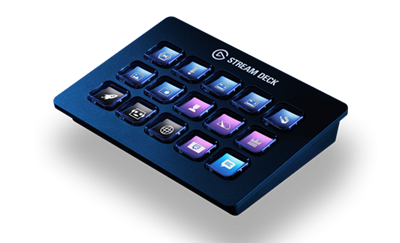
\includegraphics[width=0.5\columnwidth]{liveclips/figures/streamdeck.png}
  \caption{The Stream Deck is a programmable control pad used by many streamers, including \textit{P1}, for easy access to common shortcuts and actions. It integrates with Open Broadcaster Software (OBS), a program used by many streamers to host their live streams (\href{https://www.elgato.com/en/gaming/stream-deck}{\nolinkurl{elgato.com/en/gaming/stream-deck}}).}~\label{fig:livestream_streamdeck}
  \vspace{-0.2in}
\end{figure}

\textit{P2} is a video editor and creator who has been making video tutorials on photo and video editing for about 7 years. He hosts a podcast where he interviews people about their creative approach and life stories. He has tried Periscope, and began streaming on YouTube when it enabled mobile streaming in 2017: casual streaming was on the rise. Occasionally he live streams on YouTube or Instagram, answering viewer questions, teaching a particular topic, analyzing a popular video, or critiquing viewers' work. His setup comprises a camera view of his face, a screencast of his work, and a large monitor for him to see chat activity and other information.

\textit{P3} is a musician who live streams on Facebook and Instagram (with three band members). Her streams are spontaneous and improvisational; the quartet does not play together regularly but they have a fan base that they stream to whenever they are together. These streams require little setup; they are broadcast from a single mobile phone either held by a friend or propped up. She also occasionally streams product reviews and behind-the-scenes views of her shows.

\textit{P4} and \textit{P5} are hobby artists who stream digital drawing about once a month on Twitch. They both started streaming 2 or 3 years ago. \textit{P5} used to stream on Picarto, and moved to Twitch about a month ago because it was easier to use and tends to attract more viewers as a better-known platform. \textit{P5} rarely talks out loud during her streams (only when nobody else is home) and \textit{P4} never does. Instead, they engage with viewers by typing in the chat. Neither shows their face when streaming; their setups include only a screencast of their drawing window. 

\textit{P6}, \textit{P7}, and \textit{P8} stream as part of their jobs at Adobe by hosting artists, streaming their own work, and teaching Adobe products.
%are all employees of Adobe who regularly stream on Adobe's Daily Creative Challenges, and also host on Adobe Live. 
%These participants stream frequently as part of their jobs, and are all highly experienced at the creative work they stream. 
\textit{P6} has been making video tutorials on photo editing for over 10 years. He briefly tried streaming on Twitch but found that his audience did not transfer over to the new platform. He has been streaming with Adobe for approximately 6 months. \textit{P7} taught courses and training programs on design and illustration software for many years. He has been working at Adobe for 9 years, and streaming with Adobe for about 4 years. 
%\textit{P7} was one of the first evangelists involved in Adobe's live streaming efforts, which started on Twitch.
\textit{P8} is a designer and trained illustrator and has been streaming with Adobe for 4 years. Before joining Adobe, she used to occasionally stream her art process on Twitch. By virtue of live streaming professionally, all three participants have fairly sophisticated technology setups, including a camera view of their face in front of a green screen, a screencast of their computer, several displays for them to see chat activity and other information, and sometimes additional cameras (\autoref{fig:livestream_adobelive_setup}). 

\begin{figure}[t!]
\centering
  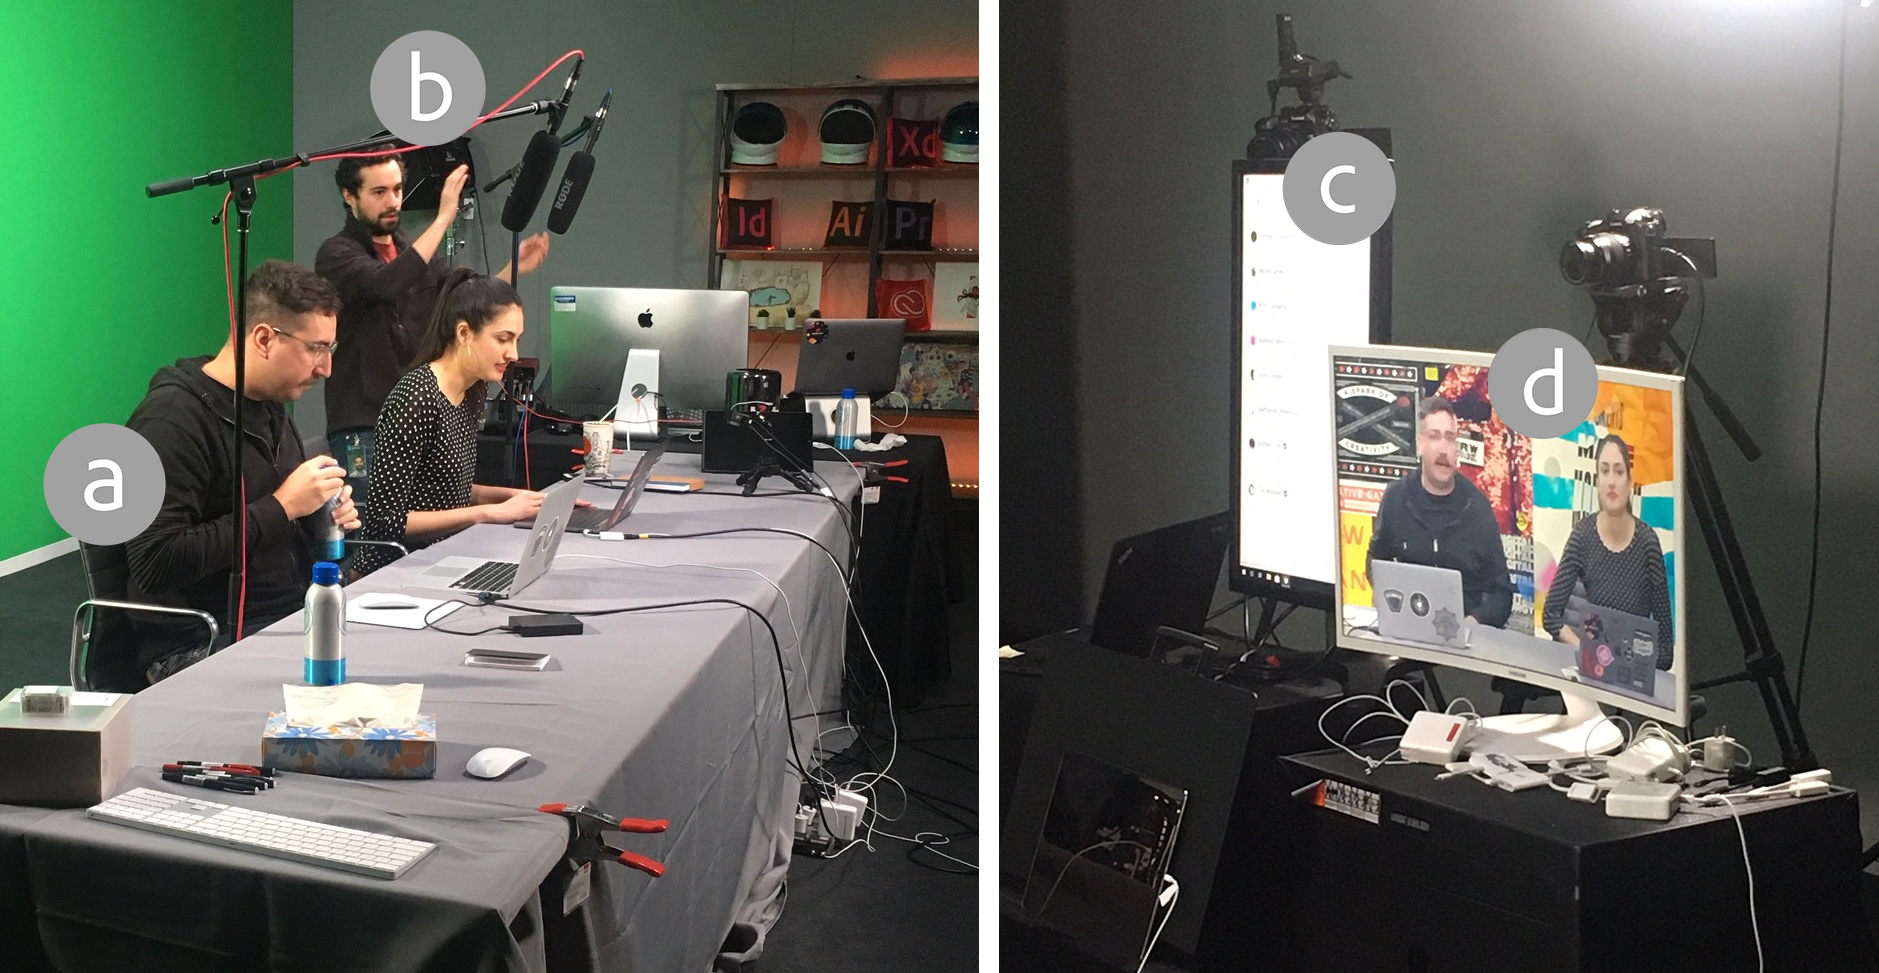
\includegraphics[width=0.8\columnwidth]{liveclips/figures/adobelive_setup.png}
  \caption[The technical setup for \textit{Adobe Live}.]{The technical setup for \textit{Adobe Live}. (a) The artist (left) and host (right) sit in front of a green screen, with both computers connected for screencasting. (b) Behind the scenes, at least one person helps with technical support, including setup, testing, and monitoring. (c) The artist and host see a display with the live chat feed, and (d) a display showing how they currently appear in the live stream. }~\label{fig:livestream_adobelive_setup}
  \vspace{-0.2in}
\end{figure}

\subsection{Findings}
\subsubsection{Audience engagement is a primary goal for streamers}
Like with gaming \cite{Pellicone2017, Hamilton2014} and culture-sharing \cite{Lu2019} live streams, audience engagement is important to creative streamers. All participants said they engage with their audience during streams, despite their different personalities and streaming styles. When asked about their main motivation for streaming, participants mentioned creating a space for people to hang out together, building an audience, sharing their process with others, and engaging in meaningful conversations.

When asked for an example of a rewarding or enjoyable moment, every participant mentioned audience engagement in some way. Three participants mentioned feeling rewarded by gratitude from viewers for inspiration and community. This inspiration goes both ways: \textit{P5} mentioned that she has received valuable feedback from a viewer that helped improve her own work. Two participants valued that \textit{``there's something more authentic about [live streaming] ... it allows me to just be myself more authentically and people can pick up on that, they can understand what you're really about in a way that you just can't express via [other modalities]''} (\textit{P2}). \textit{``There are really no mistakes, there's just honesty''} (\textit{P3}).

A key difference between gaming and creative live streams affecting engagement is the scale of the audience. The average live audience size for our participants ranged from about 5 to 1000, with most sitting at the lower end. Popular streamers of video games such as Fortnite or League of Legends often average audiences of between 2000 and 40,000. This means that creative streamers often feel a tighter personal connection with their viewers, while viewers of gaming streams tend to mostly interact with each other, as the chat goes too quickly for the streamer to keep up \cite{Lessel2017, Hu2017}.

\textit{P7} expressed a desire to offer the audience more diverse interactive experiences beyond just text chat. Currently, gaming live streams sometimes host ``audience participation games'' \cite{Glickman2018}. \textit{P1} often organizes games during live streams, such as contests with prizes, voting on what she should do next, or ``prompt games'' where viewers contribute ideas. \textit{P4} did a ``request stream'', where he drew whatever viewers requested, and \textit{P2} often runs Q\&A-form streams, where he will open an application and just let the audience ask questions. As he put it, \textit{``I want to do what they want to do.''} \textit{Adobe Live} often has giveaways for audience participation, and Adobe hosts a \textit{Daily Creative Challenge}. This kind of engagement \textit{``make[s] it a collaborative thing''} (\textit{P6}), increasing audience investment.

One emerging practice is live streaming portfolio critiques. Like a call-in radio show or newspaper advice column, a few people get direct feedback, and many people benefit through over-the-shoulder learning. This form of learning can be extremely beneficial \cite{Lopez2010}; it is notable that there is a streaming audience that seeks it out. Similar to shows and columns, streamers have the challenge of selecting which submission(s) to critique. \textit{P2} initially handled this with chat but was quickly overwhelmed by the number of messages. To address this, he found and installed a widget\footnote{\href{https://streamlabs.com/widgets}{\nolinkurl{streamlabs.com/widgets}}} to help him select submissions and allow users to pay a small amount to have their work critiqued. While valuable, it takes time and effort to manage such tools. This also exacerbates streaming's already ``fragmented technology ecosystem'' \cite{Lu2019}.

Aside from the three Adobe participants who stream as part of their jobs, none of the participants currently stream as a major income source. Though these participants were not \textit{primarily} motivated by monetary gain, two mentioned that it was a significant secondary benefit, \textit{e.g.}, \textit{P4} said, \textit{``it doesn't matter how good my work gets if I don't actually market myself.''} Many streamers in other domains (especially video games) also aim to grow their audience and make money \cite{Pellicone2017}. \textit{P1}'s sought to eventually be a self-sustaining artist; she emphasized that her primary goal was building the audience and creating a positive community; \textit{``I believe that the audience brings [financial benefits].''} \textit{P3} wished it was easier for viewers to donate. Compensation is possible on some platforms (\textit{e.g.}, Twitch) but requires configuration.

\subsubsection{Moderators \& hosts alleviate common challenges for artists}
A big part of engaging with the audience is interacting via the chat window with viewers' questions, comments, and feedback. 
%interesting: this is indirect engagement
Most participants said they sometimes have trouble keeping up with the chat as it requires switching focus from their creative work. This split-attention challenge echoes previous findings for programming \cite{Faas2018} and culture-sharing \cite{Lu2019} streams.
%- Paying attention to chat and interacting with audience while working \cite{Faas2018}, especially when work is not on the computer \cite{Lu2019} \\
%-- Messages distracting from work, especially when lots of viewers \cite{Lu2019}
\textit{P5} even said, \textit{``I usually put a warning beforehand that I'm not the most talkative while I'm drawing but I try to check up on the chat as often as I can.''} For \textit{P3} who streams on  a smartphone, it is even harder to pay attention to chat, as it requires stopping her performance and coming up close to the camera.

Moderators are one way to alleviate this challenge for viewers. In large gaming live streams, trolling is common; many streamers have dedicated moderators whose main role is to ban or time-out people posting inappropriate content and enforce a streamer's community guidelines \cite{Seering2017, Lo2018, Seering2019, YvetteWohn2019}. Trolls are seen less often in smaller live streams, yet still appear; 5/8 participants have dedicated moderators. As prior work has shown  \cite{Lo2018, Seering2019, YvetteWohn2019}, employing successful moderators requires significant preparation; streamers must work with moderators to develop guidelines, and they must constantly work to make sure their judgments align. \textit{P1} and \textit{P2} echoed these challenges: \textit{P1} has spent significant time making a document of guidelines for her moderators. \textit{P2} has not, and as a result finds that their judgments do not always align: \textit{``They might want to ban someone that I think is fine, or they might not ban someone that I think should be banned.''}

While moderators can help enforce basic rules and keep the chat constructive, they usually do not support streamers' \textit{engagement} with their audience. Viewers often have questions, feedback, and suggestions for the streamer; these are easily missed. Some moderators do engage in the chat \cite{YvetteWohn2019} but they require training in order to answer questions on behalf of the streamer (\textit{e.g.}, \textit{P1}'s moderators). In addition, some streamers find it difficult to talk out loud to their viewers: both \textit{P4} and \textit{P5} said they would like to have others to talk with, as they did not want to fill the silence alone; \textit{``I'm mostly intimidated by the idea of me having to fill a lot of void space''} (\textit{P4}). While \textit{P4} used Discord and \textit{P5} sometimes used join.me for voice chat, these require extra work on the part of the streamer, and sit outside of the main live stream platform.

A different facilitation role that Adobe streams employ to address these challenges are \textit{hosts}. \textit{Adobe Live} streams feature paid hosts who keep the artist and audience engaged, help artists feel confident, and help them focus on their work. The host watches chat messages come in, says hi and responds out loud to viewers' messages, and decides which of viewers' questions to ask to the artist. As \textit{P7} put it, the host is the \textit{``representative for the chat.''} Hosts strive to keep viewers engaged by asking the chat questions and including viewers' names when they respond to them. Hosts also strive to keep the \textit{artist} engaged and talking. As \textit{P6} put it, \textit{``the last thing you want is dead silence.''} This can be difficult when the artist is shy or quiet, so hosts have picked up tricks such as asking the artist questions about themselves, choosing questions from the chat that are likely to start a conversation, and switching the feed briefly over to their computer to show a relevant tip or trick.


%xxx: commenting out for now
%- moderators can be co-present or telepresent
%- some streamers sometimes have co-present people (helping, audience, etc)

\subsubsection{Different platforms bring different audiences}
Some participants stream on multiple platforms. Some start streaming on one platform and then switch to another. This brought up interesting trade-offs between different types of live streaming platforms. Besides mobile platforms being simpler than desktop, different platforms also bring different audiences. \textit{P6} and \textit{P8} used to stream on Twitch before Adobe's live streaming community started. They explained that Twitch is a general-purpose platform dedicated to live streaming. It attracts people who generally enjoy live streams and may be interested in creative work but are less often professional. On Twitch it's harder to attract people who are less familiar with live streams, perhaps because of unique specific features such as ``emotes''; as \textit{P1} explained, \textit{``if you are in the ecosystem you're really happy with it, and if you're not in the ecosystem it's bizarre.''}

\textit{Adobe Live} is an example of a professionally-managed live\-stream aimed at a company's customers. As a result, it tends to attract aspiring designers and creatives who use the software being shown and want to learn how to produce better work. It also attracts more people who are not familiar with live streaming, as it is shown on platforms that also include other forms of media (Behance and YouTube). A challenge with platforms like this is that \textit{``people might not really get ... why watch a live stream''} (\textit{P2}), as it is not yet widely understood.

Finally, platforms like Picarto focus specifically on \textit{creative} live streaming. These attract viewers dedicated to the topic, which can make conversations more focused. The challenge with specific platforms like these (at least in an era where the phenomenon is still growing) is that fewer people have heard of them, so it can be harder to attract viewers. For this reason, \textit{P5} switched to Twitch. Indeed, Picarto generally has 100-200 streams live at any given time, which is considerably less than the Art section alone on Twitch (which has over 300).

The type of creative work being done also affects the audience. For participants who do visual art such as drawing or use creative software, their streams tend to be of the Making or Teaching type, and their audiences mainly comprise other artists or people interested in learning the skill. For \textit{P3} who streams Performing content on Facebook, her audience mainly consists of friends and fans. These viewers enjoy watching the performance and being a part of live music, but are not necessarily looking to learn music themselves.
 
%\subsection{Streaming often requires setup and preparation}
\subsubsection{Amount of preparation depends on stream type \& preferences}
While gaming live streamers can simply turn on their screencast and begin playing a game, creative streaming often requires more preparation. 6/8 participants said they prepare before beginning a live stream. Four of these primarily run Teaching streams; the other two primarily run Making streams. For Teaching streams (\textit{P2}, \textit{P6}, \textit{P7}, and \textit{P8}), the streamers spend time before the stream going over what they will show. For Making streams, \textit{P1} and \textit{P5} spend time on the early stages of their creative work. In addition to preparing content, live streaming (especially on desktop platforms) also requires technical setup. Most participants who stream on desktop platforms said this takes time: setting up cameras and microphones, organizing windows across multiple displays, and testing the output.

Most Teaching streams require some content preparation, much like how course instructors make lesson plans. Socializing streams likely require little-to-no preparation, as the content of these streams is mainly driven by conversation with viewers. For example, \textit{P2} sometimes streams casual Q\&A streams on Instagram, enjoying their spontaneous nature: \textit{``you just go live.''} For Making and Performing, preparation time depends on the streamer. Some streamers also announce beforehand when they will stream so that viewers can plan to tune in.
%i said it better. but dont remember how
For casual Performing streams like \textit{P3}'s, all she has to do is turn on the camera and position it. But rehearsed performances require practice beforehand. \textit{P4} said he typically only plans his Making streams 5 minutes before starting, and will start drawing from scratch on the stream. \textit{P8}, who used to do more Making streams, also did not prepare: \textit{``it's as if I am opening up my sketchbook and my friends are there.''} Other Making streamers like \textit{P1} and \textit{P5} prefer to start their work before beginning a stream.

Several participants emphasized that some activities make for more engaging live streams than others. Both \textit{P1} and \textit{P5} said their streams are most successful when they do initial sketching beforehand, then spend the stream filling it in and coloring. This is because the early ideation stages involve more problem-solving and deep thinking: \textit{``to be able to put that full energy ... to get through the failures and to find the successes -- I can't multitask it.''} \textit{P5} also felt this early stage was less appealing for audiences: \textit{``For a long while they're going to have to look at a blank sheet of white `paper' so they don't really see the sketches right away ... I think that loses their attention.''} \textit{P2}, when asked why he doesn't live stream his video editing process, he said he tried it but it was too difficult to focus: \textit{``when you're video editing you need to listen to music and focus ... when you're streaming you need to be engaging with the chat.''} This echoes previous findings for knowledge-sharing \cite{Lu2018a} and programming \cite{Faas2018} streams; streamers often prepare beforehand to ensure that the content being streamed will be entertaining for viewers and will not require too much focus on the streamer's part. 

% other challenges:
% -- Delay between video and chat \cite{Lessel2017} \\
% - Entertaining both novice and expert viewers \cite{Faas2018}
% - fragmented technology ecosystem, hard to manage everything \cite{Lu2019}
% - narrating while also focusing on work \cite{Faas2018} \\
% -- Balancing entertainment with showing realistic process \cite{Faas2018} \\

\subsubsection{Permanence of live stream archives affects performance}
We found that the ability to archive live streams significantly affects how streamers perform. Several interviewees mentioned that attentiveness to viewers of a future recording influenced their choices in the moment. \textit{P7} said he sometimes records learning-focused live streams that are meant to be useful as replays, and he interacts less with viewers during those streams. \textit{P2} often deletes or hides his completed live streams because they look less polished than his regular tutorial videos. 
\textit{P4} and \textit{P5} don't archive their videos, as \textit{``[live streaming is] more of a in-the-moment [thing]''} (\textit{P5}).





\section{Open Questions and Opportunities}
This chapter's interviews as well as Chapter \ref{chapter:liveclips}'s surveys uncovered several challenges many streamers and viewers face, often due to a mismatch of goals between streamers, viewers, and existing streaming platforms. In this section, we highlight areas for future research by asking three open questions.

\subsection{How might creative live streams better engage viewers?}
In line with prior work, we found that creative streamers primarily interact with audiences through live text chat. Most interview participants mentioned difficulty keeping up with this chat, even though these streams are generally much smaller than video gaming streams. Sometimes, conflicting viewer goals can hinder the chat experience. Learners' questions can get lost in the many lines of text written by viewers who are there for social engagement. 
Streamers often enhance chat interaction using chat bots (one popular example is Nightbot\footnote{\href{https://nightbot.tv/}{\nolinkurl{nightbot.tv}}}) and install widgets to provide contests and other interactivity, but these take extra work to create, integrate, and manage.

\subsubsection{Augment chat functionality}
One approach for enhancing streamer-audience engagement might be to provide separate channels for different types of chat (as one survey participant suggested). For example, learners could post questions in one channel while social banter happens in another.

Another approach could be to design more ways for viewers to communicate beyond text. Novel streaming interfaces allow audiences to participate in video games alongside a streamer, by drawing directly on the streamer's screen to suggest moves and voting on the streamer's next move \cite{Lessel2017}, or even participating directly in the game as a side character \cite{Glickman2018}. Creative live streams may especially benefit from similar interactions. For example, viewers could annotate a streamer's work directly to ask a question about a particular section or provide feedback. Streaming platforms could also make it easier for streamers to set up polls without needing to spend too much extra time preparing them (\textit{e.g.,} detecting when the streamer poses a question and automatically creating a poll).

\subsubsection{Democratize the role of a host}
As our interviews demonstrated, having an extra person present on a stream as a host can be immensely helpful for artists. Having someone always watching the chat can alleviate this responsibility from the streamer when there are a large number of viewers, but even when viewership is small, having someone to ask questions and engage the artist in discussion can help keep a stream interesting. While moderators can address some of these challenges, by current conventions they typically do not, and not all streamers have the time or experience to find and train reliable helpers (\textit{e.g., P2}). How might we democratize the experience of having supportive hosts or facilitators?

One solution could be to take advantage of the auditory modality to mitigate the limited attention and screen space that streamers have when focusing on creative work. \textit{P4} suggested a text-to-voice service to read out chat messages so he doesn't have to look up from his work to answer questions, but noted that such a service would need to understand his own preferences so it could appropriately ``triage'' the chat, highlighting only important or relevant questions and comments. Such a system might also help streamers feel more like they are participating in a conversation rather than one-way communication.

Another challenge is to create systems to help streamers troubleshoot their technical setup in lieu of trusted moderators or hosts. While streaming from mobile platforms has become as easy as pressing ``go live,'' many interview participants described spending a lot of time experimenting with technical settings to ensure that screencasts and camera views are clear and detailed, audio is on and good quality, and background music is at an appropriate volume. Three interview participants mentioned that a system that could automatically help with this setup (or give feedback on the quality of their setup) would save substantial time and effort. 

\subsubsection{Allow searching by goal}
Future work might explore how to match audiences to the right streams in the first place, like Sj{\"{o}}blom \emph{et al.} suggest for gaming \cite{Sjoblom2017a}. Current platforms typically allow viewers to find streams based on textual metadata, like the category and title. Platforms could allow streamers to make their goals for a stream explicit and searchable, so that those seeking to learn new skills could easily find Teaching streams, and those seeking to hang out with others could directly visit Socializing streams. In addition, platforms could enable or disable different modes of audience interaction depending on a stream's goals. Future research could explore what kinds of audience interaction best benefit different types of streams.
%(\emph{e.g.,} voice comments recorded by the audience may be suitable for Socializing but disruptive for Teaching).

%- looking for the right kinds of streams -- making goals explicit. Another strategy is to help people find the right streams in the first place.

% - professional vs. amateur goals
% - for amateurs, those doing art as main gig vs. side gig goals
% - say a bit about finance / money / how that changes things
% - viewers don't always get their questions answered
% - little ways for streamers to support audience involvement, platforms don't provide many ways for audiences to participate \cite{Glickman2018}
% - interaction is currently only through chat (what if you can't type? what if you miss the moment? what if you need to communicate visually?)
% - make sure to mention chatbots/games here?
% -- Current model of one linear chatroom makes peer learning hard - hard to extract higher level summaries and there is only one way to participate in the streamer's process --> \cite{Miller2017, Lu2018} \\

%\subsection{How might we support sharing different parts of the creative process?}
\subsection{How might we make creative work more ``performable''?}
Several interview participants mentioned that they were not comfortable streaming certain parts of their creative process, because they worried it would not engage the audience, or because it required their full focus. They would instead work on these parts offline to prepare for streams. Programming streamers face a similar tension between sharing their realistic process (including difficult and less-exciting parts like debugging) and keeping the audience entertained \cite{Faas2018}. Some artists (like \textit{P4}) are comfortable sharing their entire process from the beginning. For many viewers, it can be inspiring and educational to watch an artist go through the early ideation stages, but these parts of the process may need extra work to explain to audiences,
%not lend themselves as well to visual sharing, 
as they feature a lot of internal reflection and messy iteration \cite{Schon1983}. It is possible that more automated facilitation (as discussed previously) may allow artists to focus more on their work when it needs their full attention. How else might streaming platforms better support sharing \textit{all} parts of the creative process? Are there ways to make the early stages of creative work more ``performable'' for audiences? 

\subsection{How might we support watching live stream archives?}
LiveClips (Chapter \ref{chapter:liveclips}) introduced one potential way for viewing live stream archives: extracting short clips and recommending them to users in the context of their creative software. While this might help people find in-the-moment inspiration, what about people who want to learn from a Teaching stream, or catch up on their community's activity in a Socializing stream? What are other ways we might improve the viewing experience of live stream archives?

On some platforms, such as Instagram, live streams disappear shortly after they finish. On others, like YouTube and Facebook, they are re-playable archives that show up in search results alongside other videos. In between, platforms like Twitch archive videos for a limited time (14 or 60 days depending on account type); these archives are rarely re-watched  \cite{Jia2016}, as the affordances for finding them are limited.
%Indeed, Jia et al. \cite{Jia2016} found that most video game streams are forgotten soon after they are archived. 
While popular live streams on YouTube continue to accrue views after they are archived, several survey participants (\autoref{sec:liveclips_formative}) mentioned the viewer experience is poor because the videos are long, have limited navigation, and include long periods of downtime and conversation with the then-live chat \cite{Lu2018}. Twitch viewers can create ``clips'' and streamers can create ``highlights'' of interesting moments, but they must remember to do so, and such moments can seem out-of-context when viewed on their own.

In recent work \cite{Fraser2020}, we introduced a method for automatically segmenting live stream archives into navigable sections based on the streamer's creative process. Such segmentations may help viewers more easily find specific sections in a live stream archive or glean a quick summary of what happened without needing to watch the entire video. As another example, StreamWiki \cite{Lu2018} enables viewers to collaboratively summarize a Teaching stream as it occurs. Future work should continue to explore novel ways for browsing and navigating creative live stream archives as they become increasingly prevalent online.

\section{Acknowledgements}
This chapter, in part, includes portions of material as it appears in \textit{Sharing the Studio: How Creative Livestreaming can Inspire, Educate, and Engage} by C. Ailie Fraser, Joy O. Kim, Alison Thornsberry, Scott Klemmer, and Mira Dontcheva in the Proceedings of the 2019 on Creativity and Cognition (C\&C '19). The dissertation author was the primary investigator and author of this paper.